\documentclass[11pt,amsmath,amssymb]{revtex4}

 \usepackage{graphicx}
\usepackage{graphics,epsfig}
 \usepackage{amssymb}
 \usepackage{ulem}
 \usepackage{multirow}
  \usepackage{color}
  \usepackage{hyperref}
  
  
  \usepackage{listings}
\usepackage{color}
\usepackage{float}

\definecolor{dkgreen}{rgb}{0,0.6,0}
\definecolor{gray}{rgb}{0.5,0.5,0.5}
\definecolor{mauve}{rgb}{0.58,0,0.82}

\lstset{frame=tb,
  language=Python,
  aboveskip=3mm,
  belowskip=3mm,
  showstringspaces=false,
  columns=flexible,
  basicstyle={\small\ttfamily},
  numbers=none,
  numberstyle=\tiny\color{gray},
  keywordstyle=\color{blue},
  commentstyle=\color{dkgreen},
  stringstyle=\color{mauve},
  breaklines=true,
  breakatwhitespace=true
  tabsize=3
}

 \def\be{\begin{equation}}
\def\ee{\end{equation}}
 \def\bi{\begin{itemize}}
 \def\ei{\end{itemize}}
  \def\ben{\begin{enumerate}}
\def\een{\end{enumerate}}
  \def\bt{\begin{tabular}}
\def\et{\end{tabular}}
\def\bc{\begin{center}}
\def\ec{\end{center}}

\linespread{1.}
\pagestyle{plain}
\usepackage{graphics}
\usepackage{color}
\usepackage{helvet}
%\usepackage{palatino}
\setcounter{section}{0}

\renewcommand{\thesection}{\Alph{section}}
\setcounter{page}{1}
\renewcommand{\thepage}{I-\arabic{page}}
\def\be{\begin{equation}}
\def\ee{\end{equation}}
\def\bea{\begin{eqnarray}}
\def\eea{\end{eqnarray}}
\def\tcr{\textcolor{red}}
\def\accent{\it}



\begin{document}
%------------------------------------------------------------------------------------------
\title{Genetic Programming}
\author{V. Hunter Adams}

\begin{abstract}
I've used a tree structure to implement a genetic program that evolves populations of mathematical functions. Below, I've used the program to fit three sets of data (an asymptotic division, a line, and a circle), both with and without noise.
\end{abstract}
\maketitle


\section{Representation}
%-------------------------------------------------------------------------------------------
Fundamentally, my GP manipulated objects of two classes that I defined: person and population. Each person is a tree of constants, operators, and variables; and the population is a list of persons. Both the person class and the population class had parameters that I could manipulate from run to run.

The knobs that I was able to turn (on the person level) included operator mutation rate (the rate at which an operator would randomly change into another operator), constant mutation rate (the rate at which constants turned into other constants), variable introduction rate (the rate at which constants turned into variables), variable outroduction rate (rate at which variables turned into constants), maximum constant (maximum allowable value for a constant), maximum depth (maximum depth of tree), and extension rate (rate at which the tree tends to grow new branches). I found some combinations of parameters that worked better than others (see below).

On the population level, I had the ability to vary elitism (the proportion of elite individuals that I kept from each generation), selection pressure, and population size.

However, this representation did lead me to some problems. Whenever the tree found the variable 'x', it would return an array of all the x points from the data files and perform all the operations in the tree on that array of x's. For explicit functions of the form $y=f(x)$ (like the div or the line), this worked very well and the GP found the solution without any problem. The same was not the case for the circle.

I will go into more depth in the Circle section of this report, but I had a huge amount of trouble getting the square root operator to work. I backed myself into a corner by using representation that demanded equations of the form $y=f(x)$, and I had trouble getting myself out of that corner. See Section D for more explanation.

To evaluate fitness, I performed a mean-square-error operation between the y-points that the GP produced and the given y-points.

\section{The Asymptotic Division}
%-------------------------------------------------------------------------------------------
\subsubsection{Without Noise}
For the asymptotic division, the GP found a solution that generated points that were indistinguishable from the target solution after ~125,000 evaluations. I ran the GP a few times, turning the knobs mentioned above for each run. See the plots below for the optimal solution that the GP found and the fitness vs. evaluations plots for each run.

For the division without noise, the GP found the solution:

\begin{equation}
y = x+\frac{0.0257}{x}
\end{equation}

Which had a mean square error on the order $10^{-3}$.


\begin{figure}[H]
\center
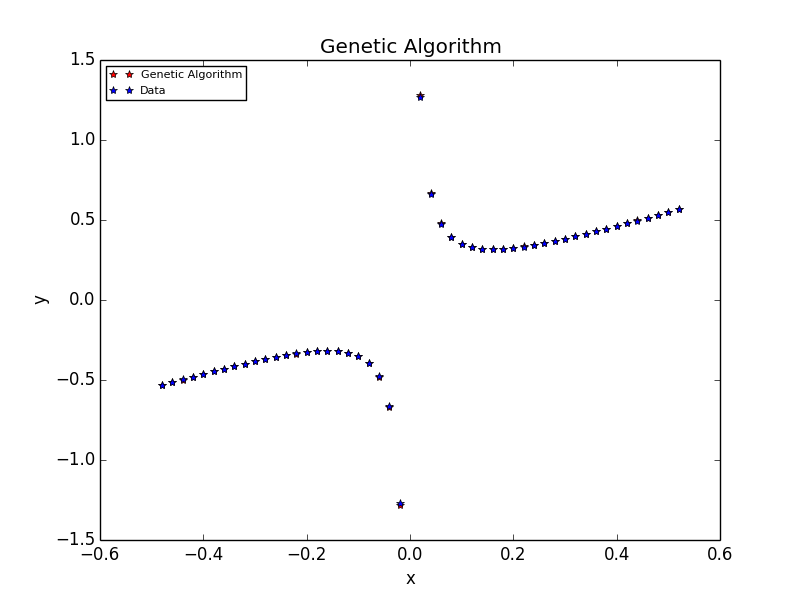
\includegraphics[scale=0.55]{Div_No_Noise.png}
\caption{Plot of the given data points and the genetically produced data points. The GP had an elitism pressure of 0.3, selection pressure of 0.4, operator mutation rate of 0.5, constant mutation rate of 0.5, variable introduction rate of 0.6, variable outroduction rate of 0.4, max depth of 100, and extension rate of 0.7. What all of that means is that the GP preferred to add variables as opposed to take them away, and it preferred to create larger trees as opposed to smaller ones.}
\label{q1}
\end{figure}

\begin{figure}[H]
\center
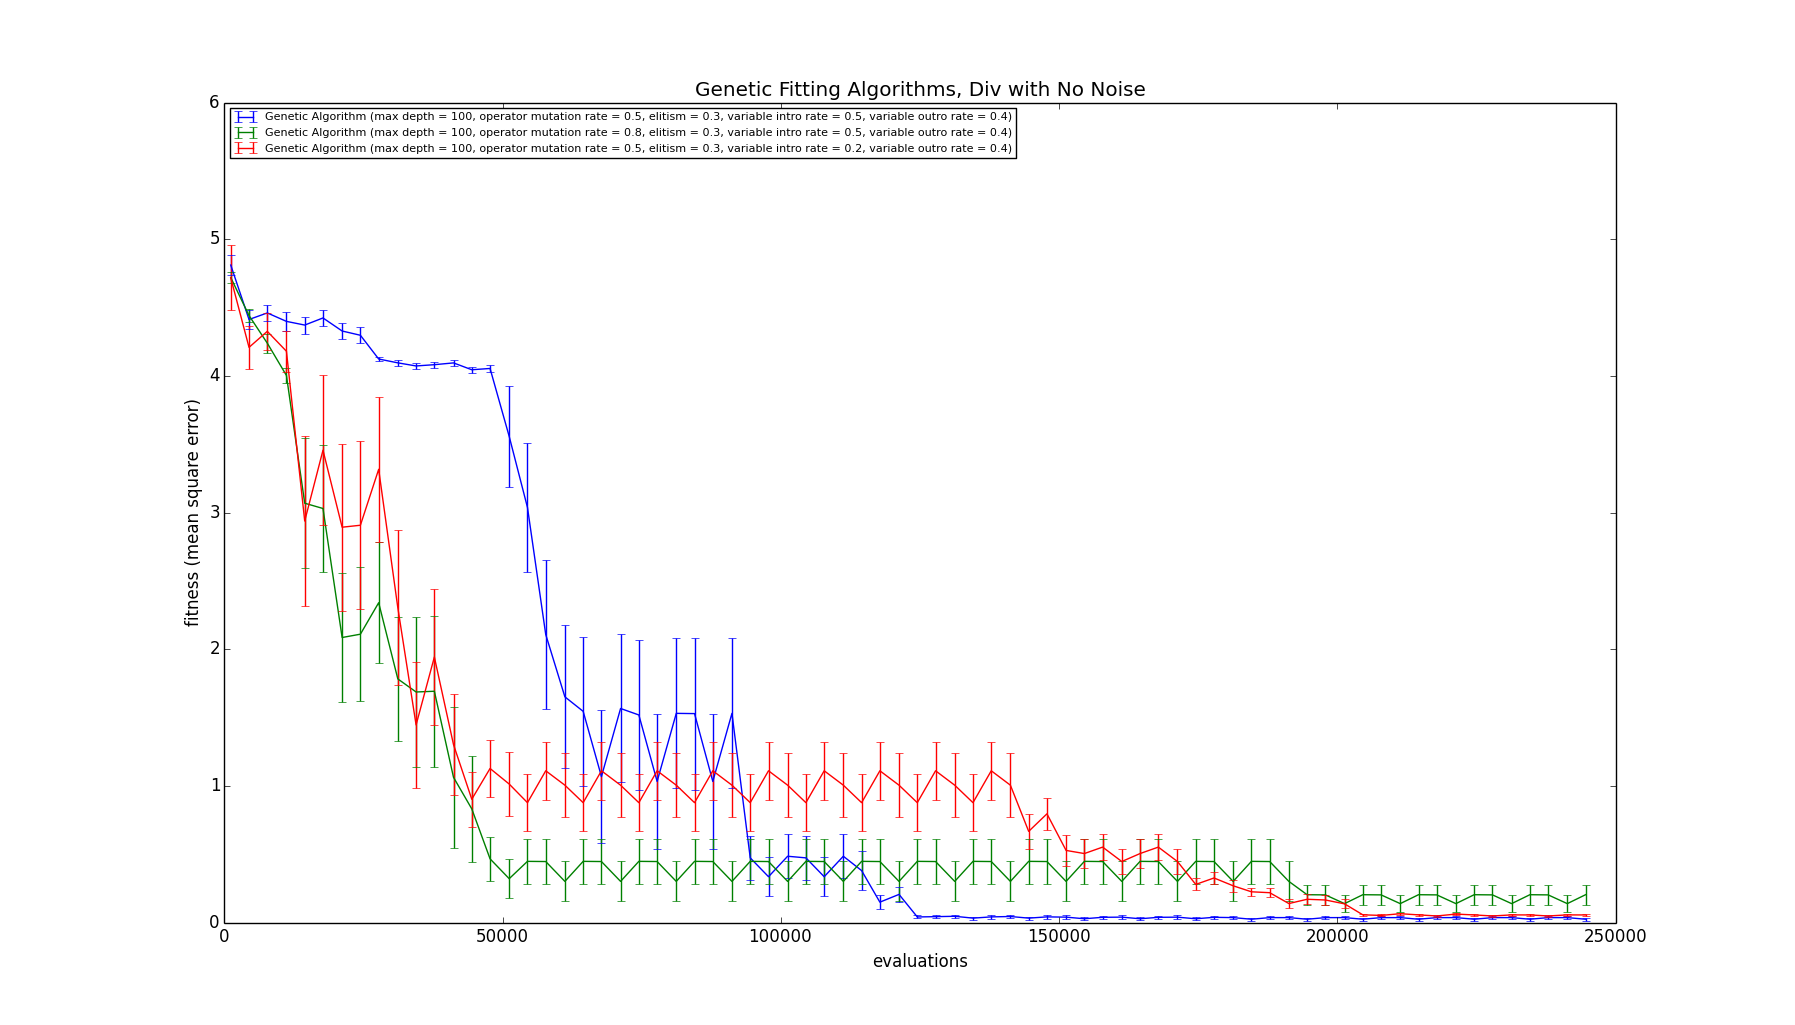
\includegraphics[scale=0.4]{Div_No_Noise_Comparison.png}
\caption{Fitness vs. number of evaluations for multiple runs of the GP on the asymptotic division with no noise, with different knobs turned different directions. Here, I varied the operator mutation rate and the variable introduction rate. In the long term, I found that the GP with variable introduction rate of 0.5, variable outroduction rate of 0.4, and operator mutation rate of 0.5 won over the GP's that were more reluctant/excited to add variables or mutate operators.}
\label{q1}
\end{figure}


\subsubsection{With Noise}
I noticed some interesting behavior with the noisy asymptotic division (and, in fact, for the noisy functions in general). The GP would place noise into some of the optimal solutions, but the best solution that it returned (the one with the lowest mean square error) was not always a noisy one. This could potentially be because I used a gaussian distribution to add noise to the function, and a set the standard deviation of that gaussian noise to 0.2 (based on inspection). It is possible that the noise that I was adding did not exactly match the type of noise in the function, and that this is why the fittest solutions were not always noisy.

I used the GP to find a solution without any domain knowledge at all, and it returned a very deep tree that fit the data very well. However, when I introduced a little bit of domain knowledge from the solution of the noiseless division (simply by restricting the depth of the tree), the search space was reduced and it eventually found a better solution. Thought the {\bf{best}} solution still did not include noise, which is clearly a problem.

The fittest solution that the GP found for the noisy data was:

\begin{equation}
noisy div equation
\end{equation}



\begin{figure}[H]
\center
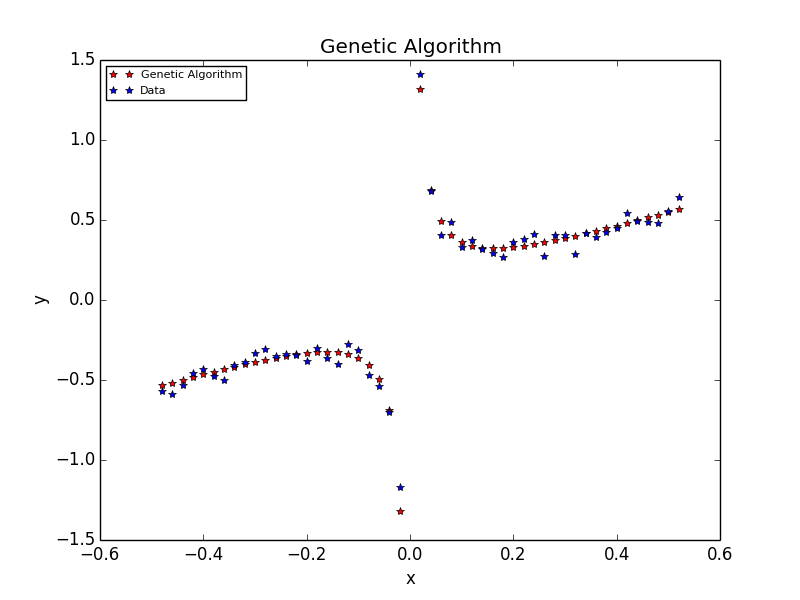
\includegraphics[scale=0.55]{Div_Noise.png}
\caption{Plot of the given data points and the genetically produced data points. The GP had an elitism pressure of 0.3, selection pressure of 0.4, operator mutation rate of 0.5, constant mutation rate of 0.5, variable introduction rate of 0.6, variable outroduction rate of 0.4, max depth of 100, and extension rate of 0.7. What all of that means is that the GP preferred to add variables as opposed to take them away, and it preferred to create larger trees as opposed to smaller ones.}
\label{q1}
\end{figure}

\begin{figure}[H]
\center
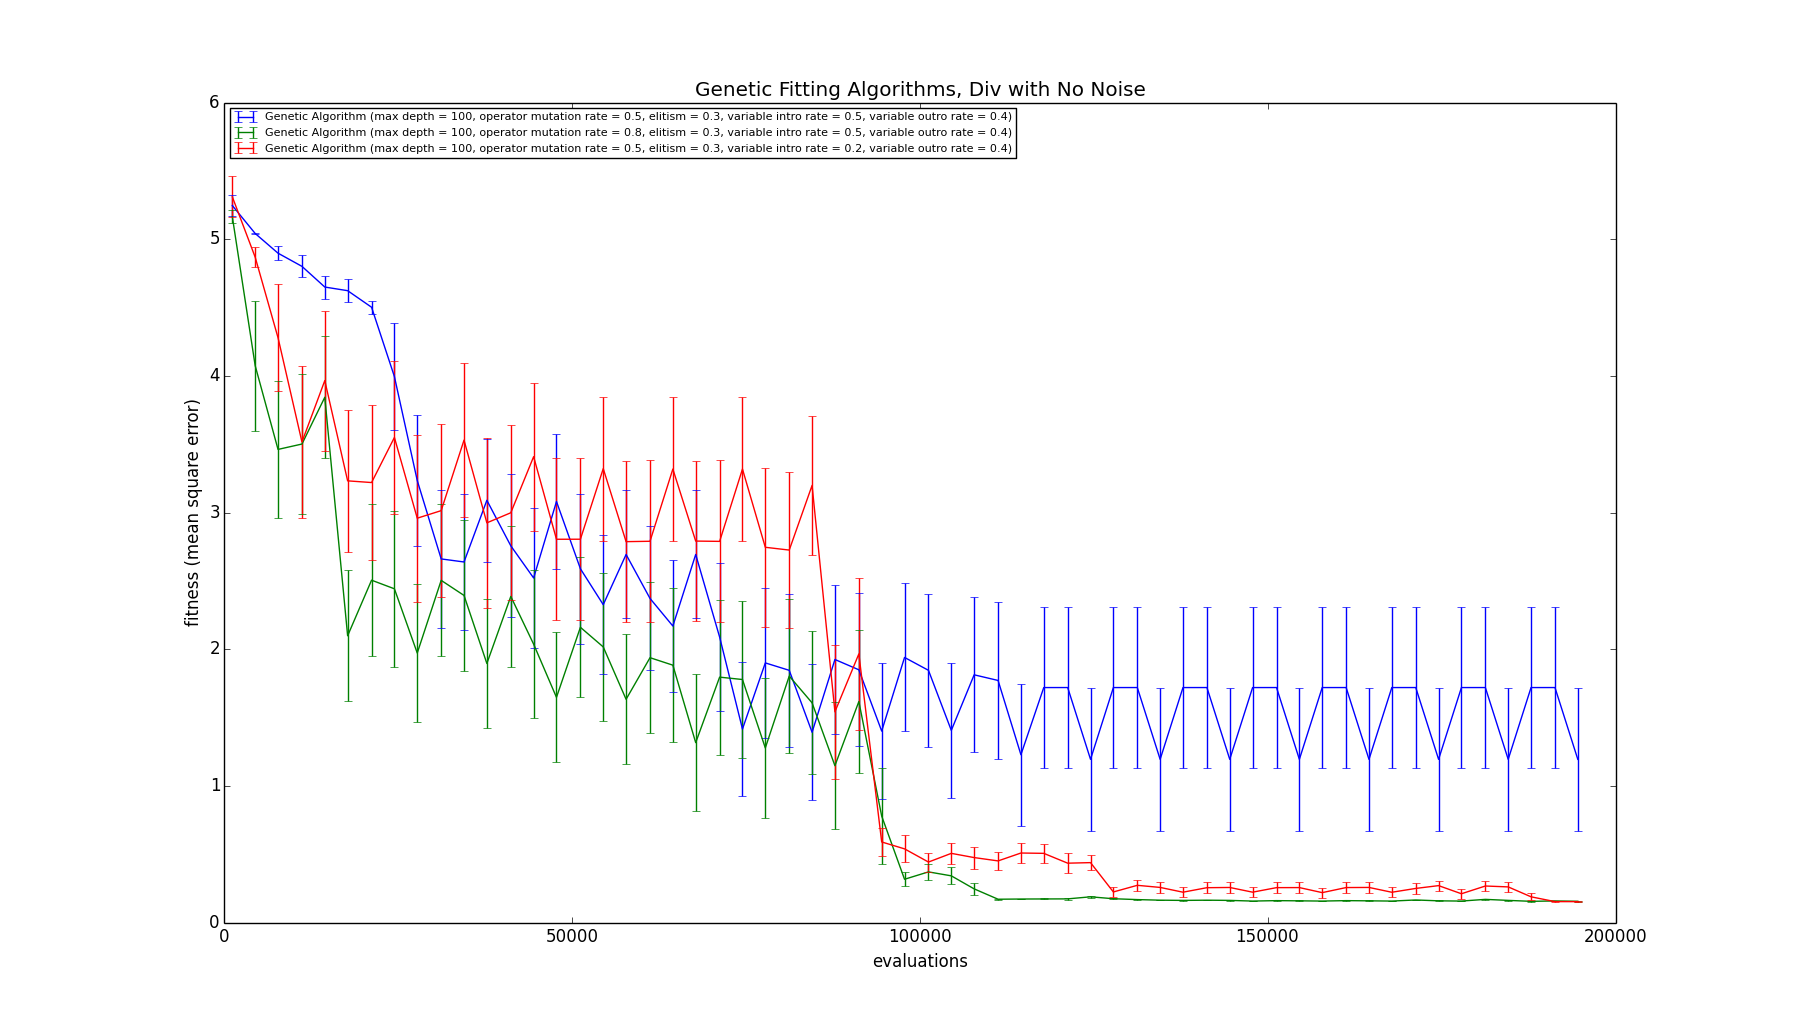
\includegraphics[scale=0.4]{Div_Noise_Comparison.png}
\caption{Fitness vs. number of evaluations for multiple runs of the GP on the asymptotic division with noise, with different knobs turned different directions. Here, I varied the operator mutation rate and the variable introduction rate. In the long term, I found that the GP with variable introduction rate of 0.5, variable outroduction rate of 0.4, and operator mutation rate of 0.8 won over the GP's that were more reluctant/excited to add variables or mutate operators. This differs from the noiseless function, which did not prefer to have its operators mutated as frequently.}
\label{q1}
\end{figure}


\section{The Line}
%-------------------------------------------------------------------------------------------
\subsubsection{Without Noise}
The noiseless line seemed to be too easy of a problem for the GP. In fact, my program would initialize itself by generating a population of 50 equations, each of depth two. I would often find that ranking this initial (random) population often returned a solution that was already pretty close to optimal. Within just a few generations, the GP found a solution that generated y points that were completely indistinguishable from the given y points (mean square error on the order $10^{-4}$) after ~1500 evaluations. I included fitness vs. evaluations plots for the line, but they are not particularly interesting to look at because this was such a simple problem for the GP.

\begin{figure}[H]
\center
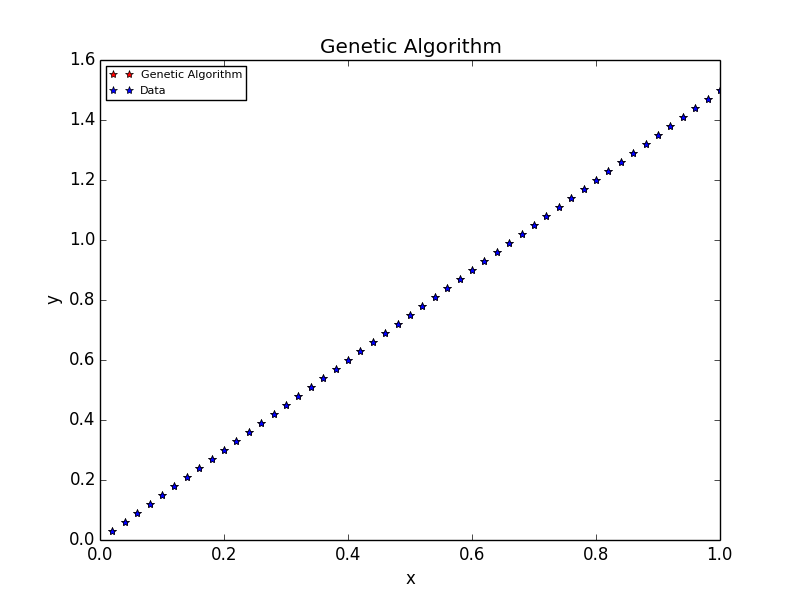
\includegraphics[scale=0.55]{Line_No_Noise.png}
\caption{Plot of the given data points and the genetically produced data points. The GP had an elitism pressure of 0.3, selection pressure of 0.4, operator mutation rate of 0.5, constant mutation rate of 0.5, variable introduction rate of 0.6, variable outroduction rate of 0.4, max depth of 100, and extension rate of 0.7. What all of that means is that the GP preferred to add variables as opposed to take them away, and it preferred to create larger trees as opposed to smaller ones.}
\label{q1}
\end{figure}

\begin{figure}[H]
\center
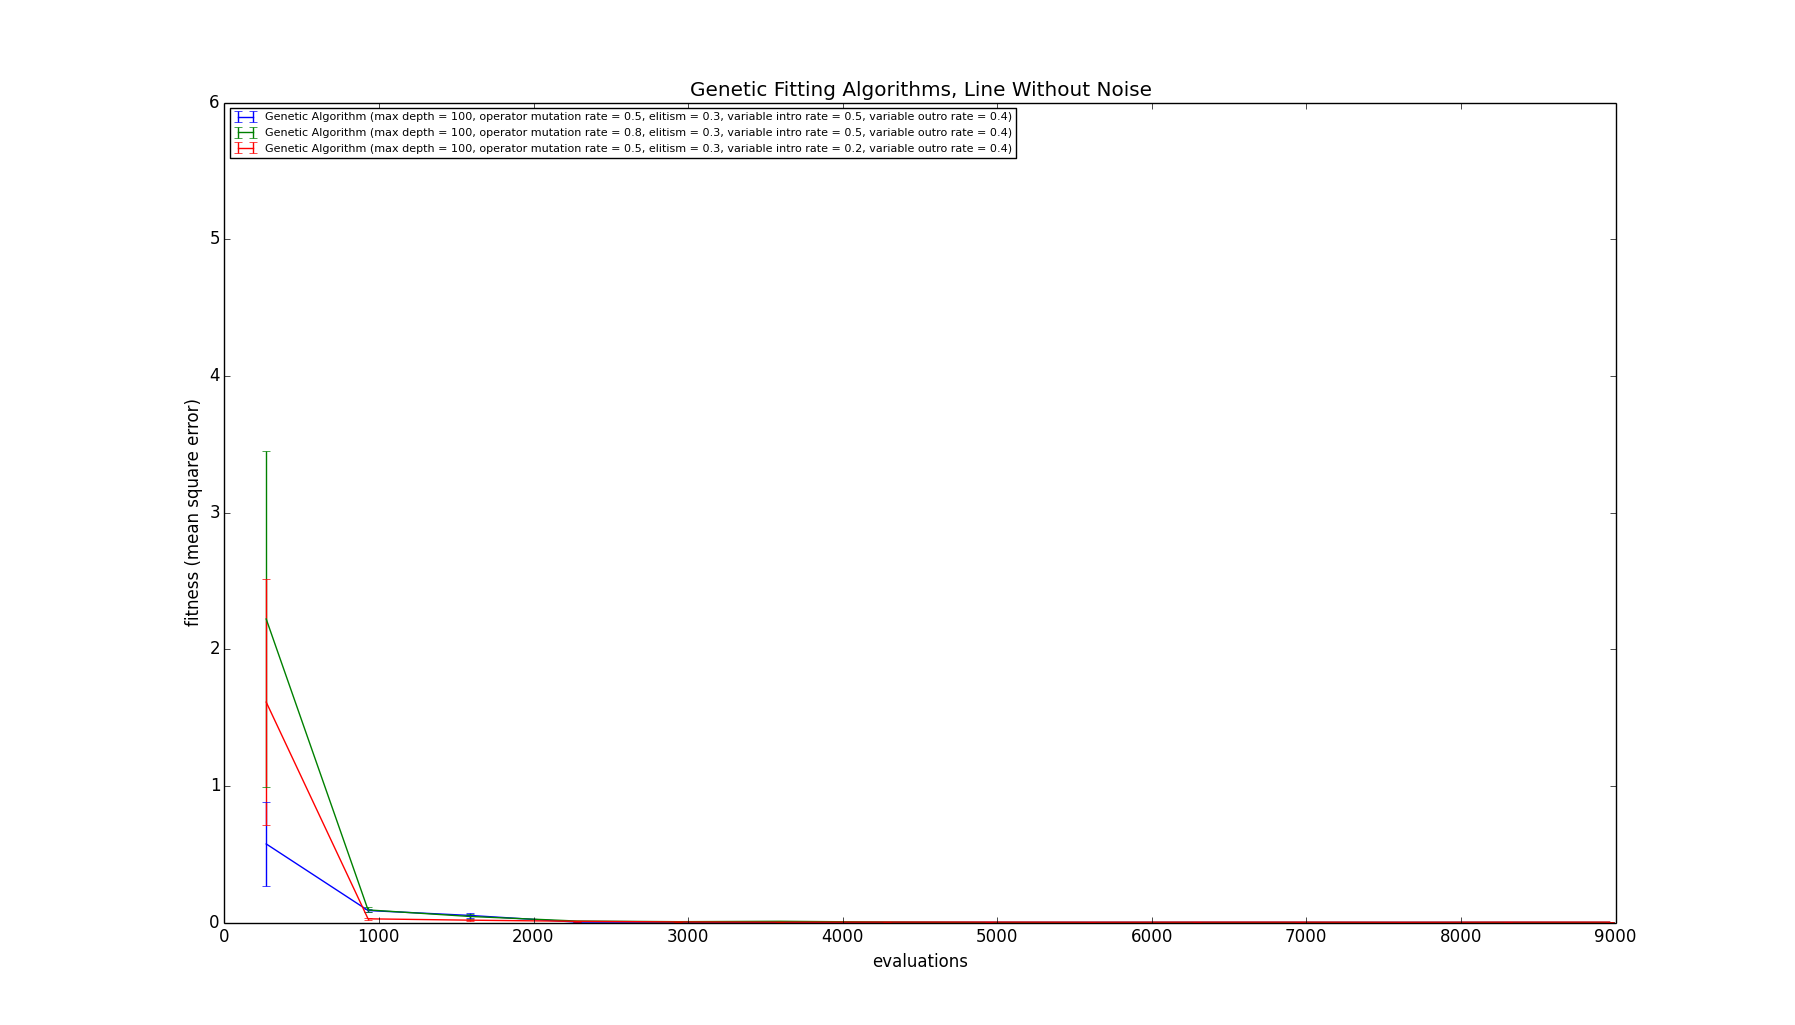
\includegraphics[scale=0.4]{Line_No_Noise_Comparison.png}
\caption{Fitness vs. number of evaluations for multiple runs of the GP on the line with no noise, with different knobs turned different directions. As I mentioned, the line does not generate particularly interesting data.}
\label{q1}
\end{figure}

\subsubsection{With Noise}
I noticed the same phenomenon with the noisy line that I noticed with the noisy asymptotic division, where the best solution generated did not include the 'noise' operator. As I mentioned previously, this could potentially be because I was adding the wrong type of noise (perhaps it was not gaussian, or perhaps the standard deviation was not 0.02). The GP still found a solution with a mean square error of 0.14, given by:

\begin{equation}
noisy equation line
\end{equation}

\begin{figure}[H]
\center
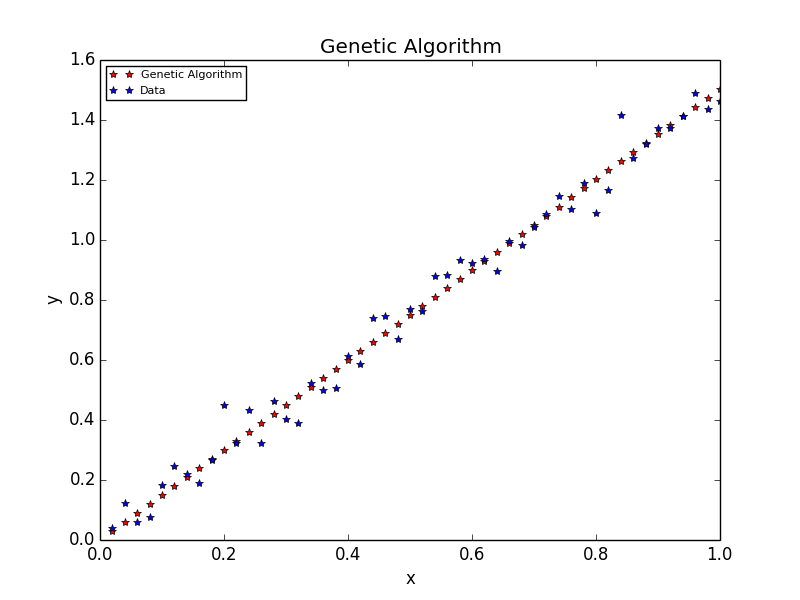
\includegraphics[scale=0.55]{Line_With_Noise.png}
\caption{Plot of the given data points and the genetically produced data points. The GP had an elitism pressure of 0.3, selection pressure of 0.4, operator mutation rate of 0.5, constant mutation rate of 0.5, variable introduction rate of 0.6, variable outroduction rate of 0.4, max depth of 100, and extension rate of 0.7. What all of that means is that the GP preferred to add variables as opposed to take them away, and it preferred to create larger trees as opposed to smaller ones.}
\label{q1}
\end{figure}

\begin{figure}[H]
\center
\includegraphics[scale=0.4]{Line_With_Noise_Comparison.png}
\caption{Fitness vs. number of evaluations for multiple runs of the GP on the line with noise, with different knobs turned different directions. As I mentioned, the line does not generate particularly interesting data.}
\label{q1}
\end{figure}


\section{The Circle: Problems Encountered and Attempted Solutions}
%-------------------------------------------------------------------------------------------
As I mentioned at the beginning of this report, I backed myself into a corner by choosing a representation of the form $y=f(x)$ for my GP. Below, I've explained each problem that I encountered and the solution that I implemented to solve that problem. In the end, the GP did not find an optimal solution for the circle. I don't feel like I wasted my time, however, because wrestling with this problem taught me a lot of lessons the (very) hard way.



\newpage\newpage
\section{My Code}
\begin{lstlisting}

\end{lstlisting}



\end{document}